% Martin Rodriguez Jr.
% SID: 811958765


%Anything following a % sign is a comment.
%Please use the comments to help you understand the code below.

%%%%%%%%%%%% Quick Notes %%%%%%%%%%%%%%%%%%%%%%

% \textit{} ==> italicises words or phrases
% \textbf{} ==> bolds words or phrases
% \\ ==> creates a new line
% \S ==> creates section section symbol, fancy double s thing
% \renewcommand{\baselinest8retch}{2} ==> double spaces the document

%%%%%%%%%%%%%%%%%%%%%%%%%%%%%%%%%%%%%%%%
\documentclass[12pt]{article}

%LOAD VARIOUS PACKAGES
\usepackage{setspace}
\usepackage{caption}
\usepackage{subcaption}
\usepackage{graphics, latexsym, multicol}		%
\usepackage{graphicx}
\usepackage{lscape}

\usepackage{amsmath, amsfonts, amsthm, amssymb}		%Math packages provided by American Math Society (AMS)
\usepackage{thmtools}

\usepackage{xcolor}							%Extended color package: provides colors for text enhancement
%\usepackage[margin = 1.00in, top = 1in, bottom = 1in, nohead] {geometry}
\usepackage{boxedminipage}					%allows use of boxed minipages
\usepackage{enumitem}


\usepackage[english]{babel}
\usepackage{xcolor} % Required for specifying custom colors
\usepackage{fix-cm} % Allows increasing the font size of specific fonts beyond LaTeX default specifications

\usepackage{longtable}

%MATH CHARACTER COMMANDS: Short hand for commands
\def\N{\mathbb{N}}		 				%Natual Bold Face: \N is now the command for the Natural Numbers
\def\Q{\mathbb{Q}} 						%Rational Bold Face: \R
\def\R{\mathbb{R}} 						%Real Bold Face
\def\Z{\mathbb{Z}} 						%Integers Bold Face
\def\C{\mathbb{C}} 						%Complex Bold Face
\def\eps{\varepsilon}                                               % Defines \varepsilon to \eps
\renewcommand{\qedsymbol}{$\blacksquare$} % QED symbol

\def\L{\mathcal{L}}



%Solution template with little sideways triangle
\declaretheoremstyle[
spaceabove=6pt, spacebelow=6pt,
headfont=\normalfont\bfseries,
notefont=\mdseries, notebraces={(}{)},
bodyfont=\normalfont,
postheadspace=1em,
numberwithin=section
]{exstyle}
\declaretheoremstyle[
spaceabove=6pt, spacebelow=6pt,
headfont=\normalfont\bfseries,
notefont=\mdseries, notebraces={(}{)},
bodyfont=\normalfont,
postheadspace=1em,
headpunct={},
qed=$\blacktriangleleft$,
numbered=no
]{solstyle}
\declaretheorem[style=exstyle]{example}
\declaretheorem[style=solstyle]{solution}

%\newenvironment{solution}
%  {\begin{proof}[Solution]}
%  {\end{proof}}
%
%



\usepackage{hyperref}
\usepackage{listings}


\begin{document}

\begin{center}
	{\LARGE Homework 6} \\[10pt] 
	{ Martin Rodriguez} \\
	Student ID: 1151332\\
	AMS 209: Foundations of Scientific Computing\\
	Professor Dongwook Lee\\[10 pt]	
	29 November 2017 \\[30 pt]
\end{center}

The goal of this homework was to create a \texttt{Python} script that can compile and execute \texttt{Fortran} code. In addition, the python script also created a \texttt{.txt} file with the runtime parameters and managed output files to make sure they were not overwritten. Lastly, the \texttt{Python} code also grabs the \texttt{.dat} files and plots the results.

The \texttt{Fortran} code performs the Newton's method to find the roots of a specific function with the given threshold. In this case we use
\begin{align}
	f(x) = (x-1)\log_{10}(x).
\end{align} 
The root of the problem is $x^* = 1$ then we test the code using two different initial guesses $x_0 = 1.2$ and $x_0 = 0.0001$. As can be seen in the following figures, the error for the initial guess near the root is very small. However, for the solution far away from the root begins small then shoots up and once again falls down below the threshold.  

\newpage
\section*{{\large Initial Condition $\boldsymbol{x_0 = 1.2}$}}
	For threshold  error 0.0001:
	\begin{figure}[h]
		\caption{The target function $f(x) = (x-1)\log_{10}(x)$.}
		\centering
		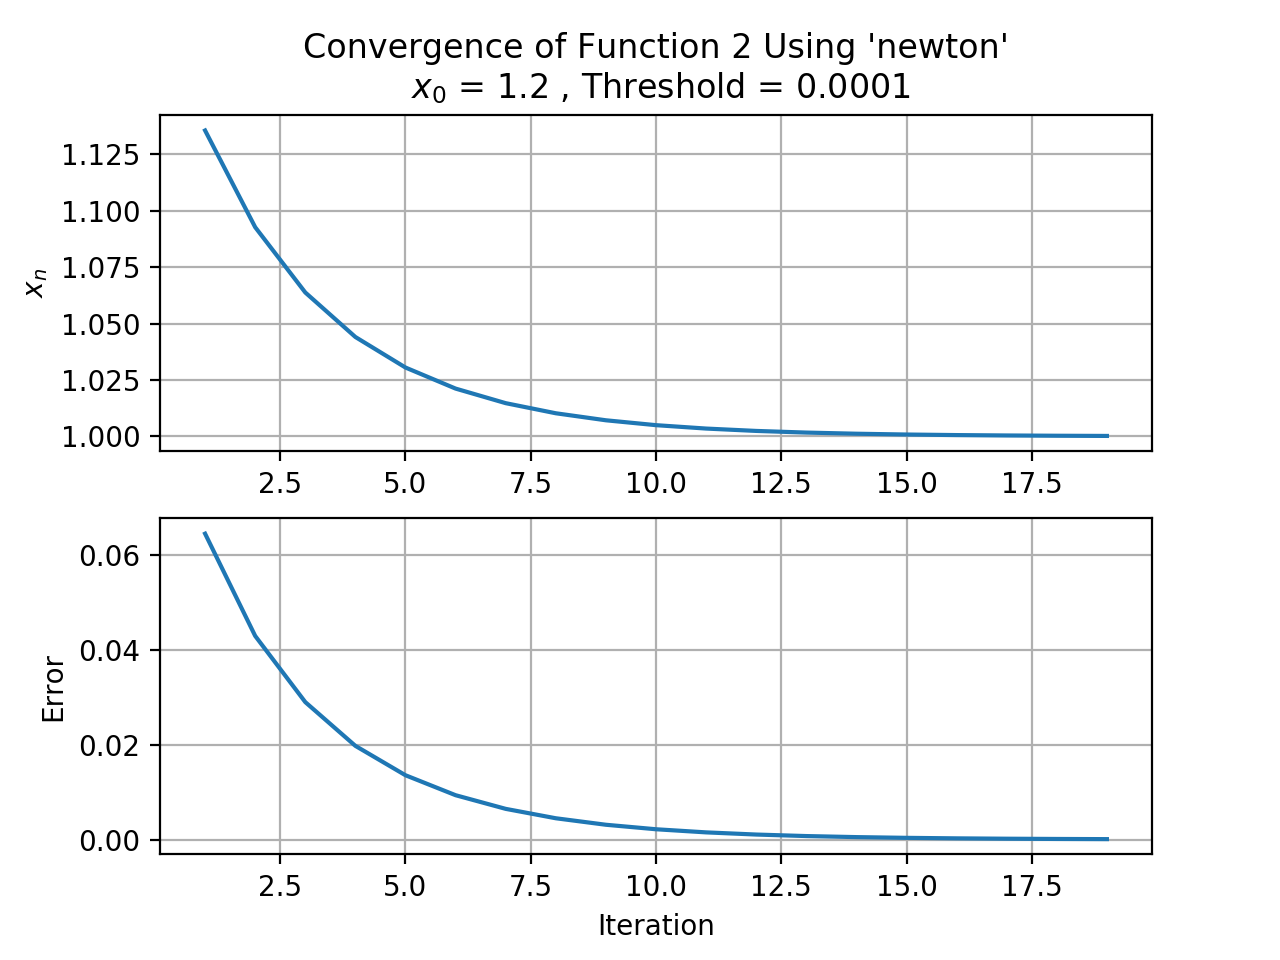
\includegraphics[width=1.0\textwidth]{./figures/initial_condition_1/result_2_0001.png}
		\label{fig:plot2dot3}
	\end{figure}
	
	\newpage
	For threshold  error 1.0e-6:
		\begin{figure}[h]
		\caption{The target function $f(x) = (x-1)\log_{10}(x)$.}
		\centering
		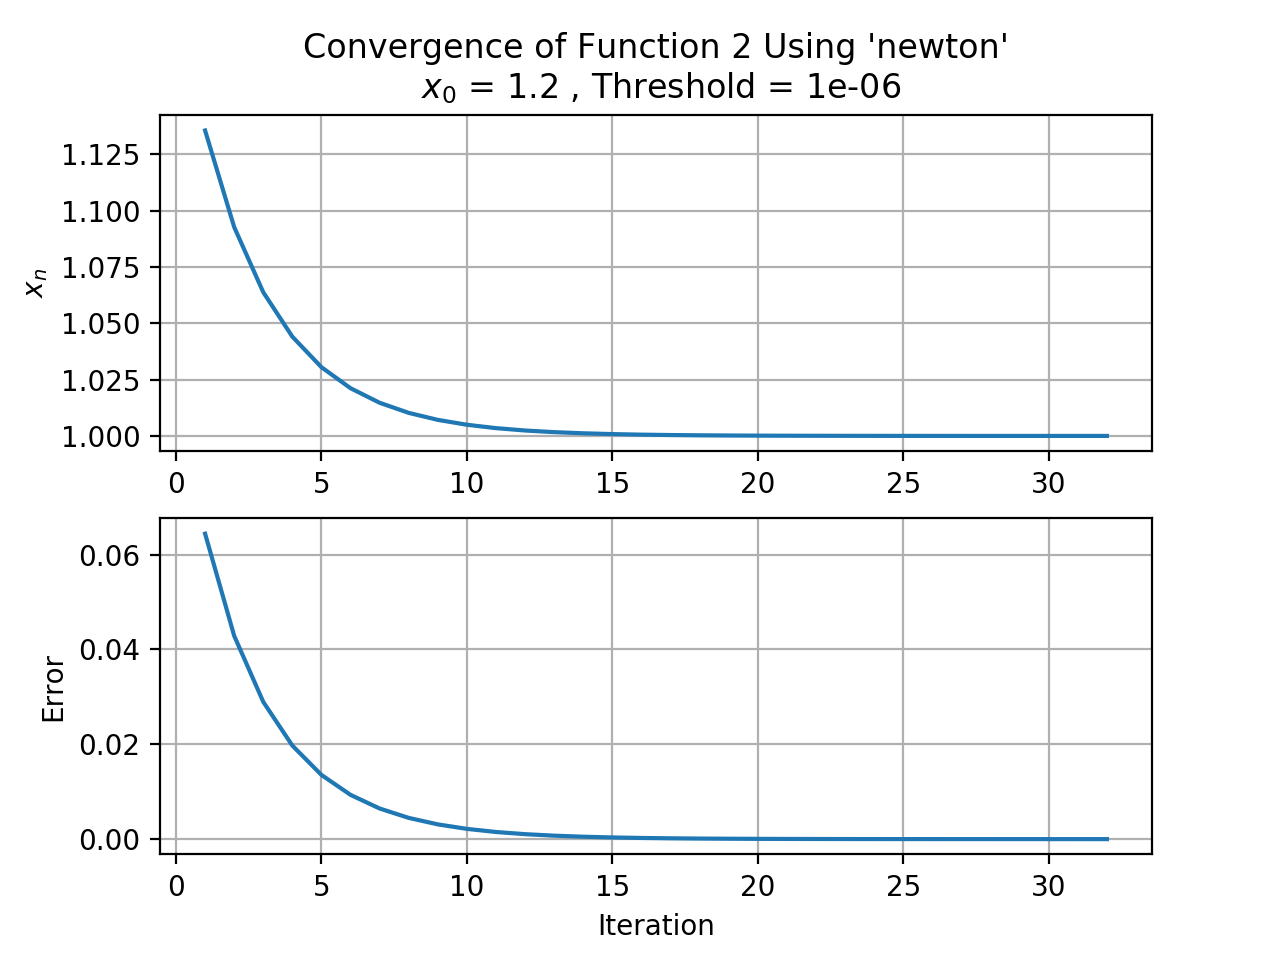
\includegraphics[width=1.0\textwidth]{./figures/initial_condition_1/result_2_1e-06.png}
		\label{fig:plot2dot3}
	\end{figure}
	
	\newpage
	For threshold  error 1.0e-8:
		\begin{figure}[h]
		\caption{The target function $f(x) = (x-1)\log_{10}(x)$.}
		\centering
		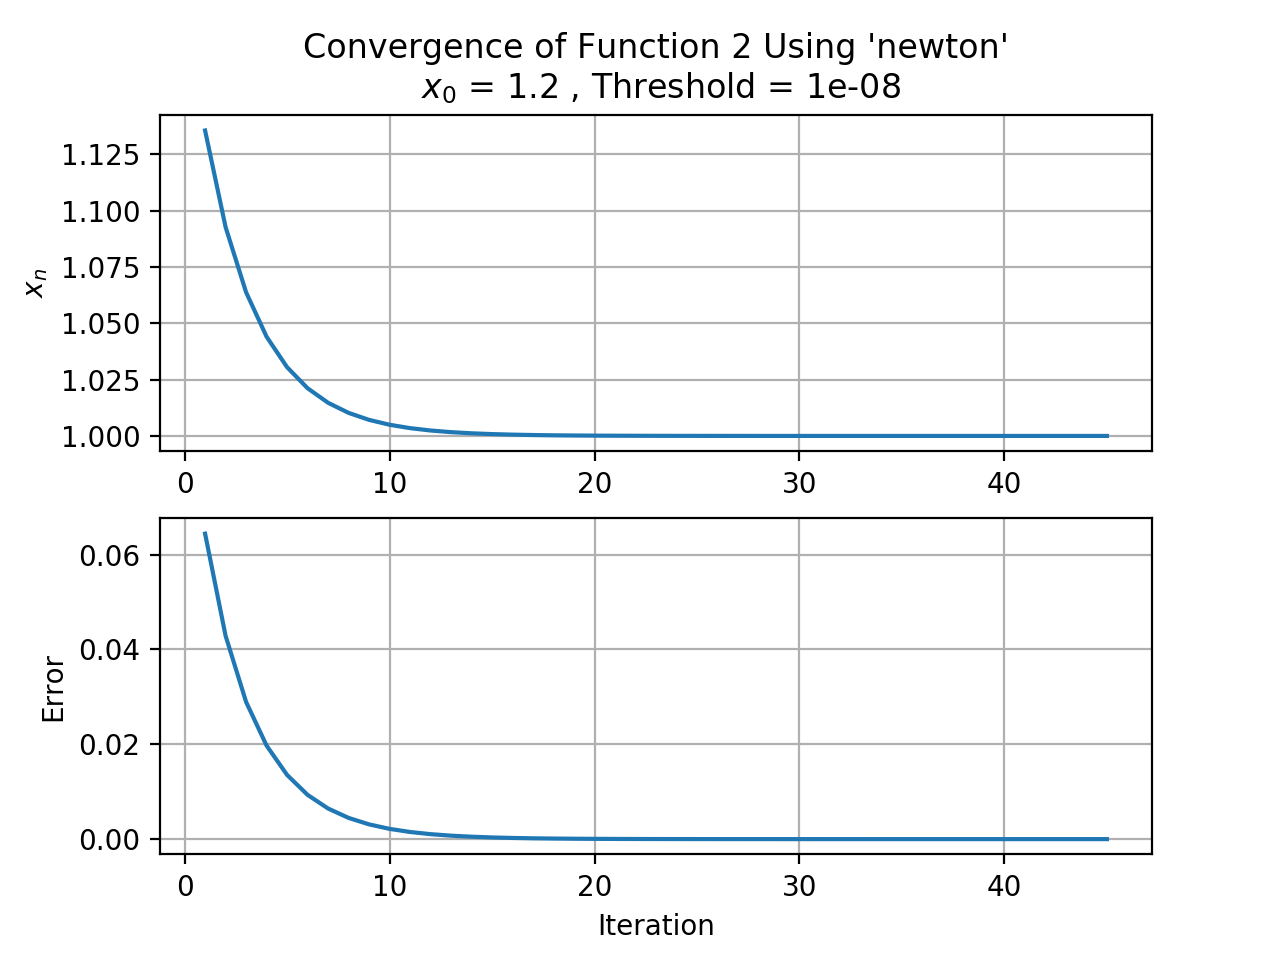
\includegraphics[width=1.0\textwidth]{./figures/initial_condition_1/result_2_1e-08.png}
		\label{fig:plot2dot3}
	\end{figure}





\newpage
\section*{{\large Initial Condition $\boldsymbol{x_0 = 0.0001}$}}
	For threshold  error 0.0001:
	\begin{figure}[h]
		\caption{The target function $f(x) = (x-1)\log_{10}(x)$.}
		\centering
		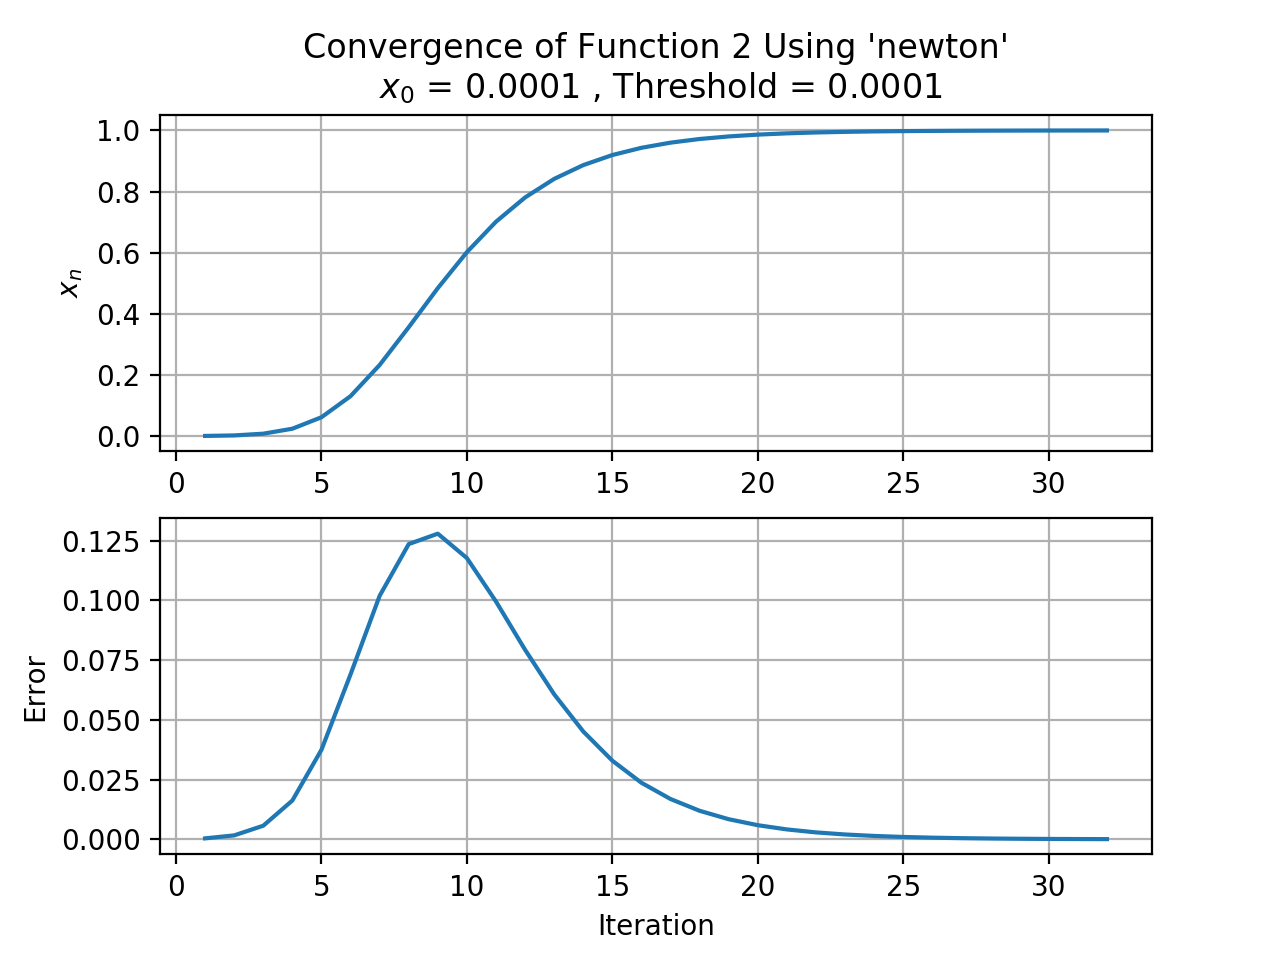
\includegraphics[width=1.0\textwidth]{./figures/initial_condition_2/result_2_0001.png}
		\label{fig:plot2dot3}
	\end{figure}
	
	\newpage
	For threshold  error 1.0e-6:
		\begin{figure}[h]
		\caption{The target function $f(x) = (x-1)\log_{10}(x)$.}
		\centering
		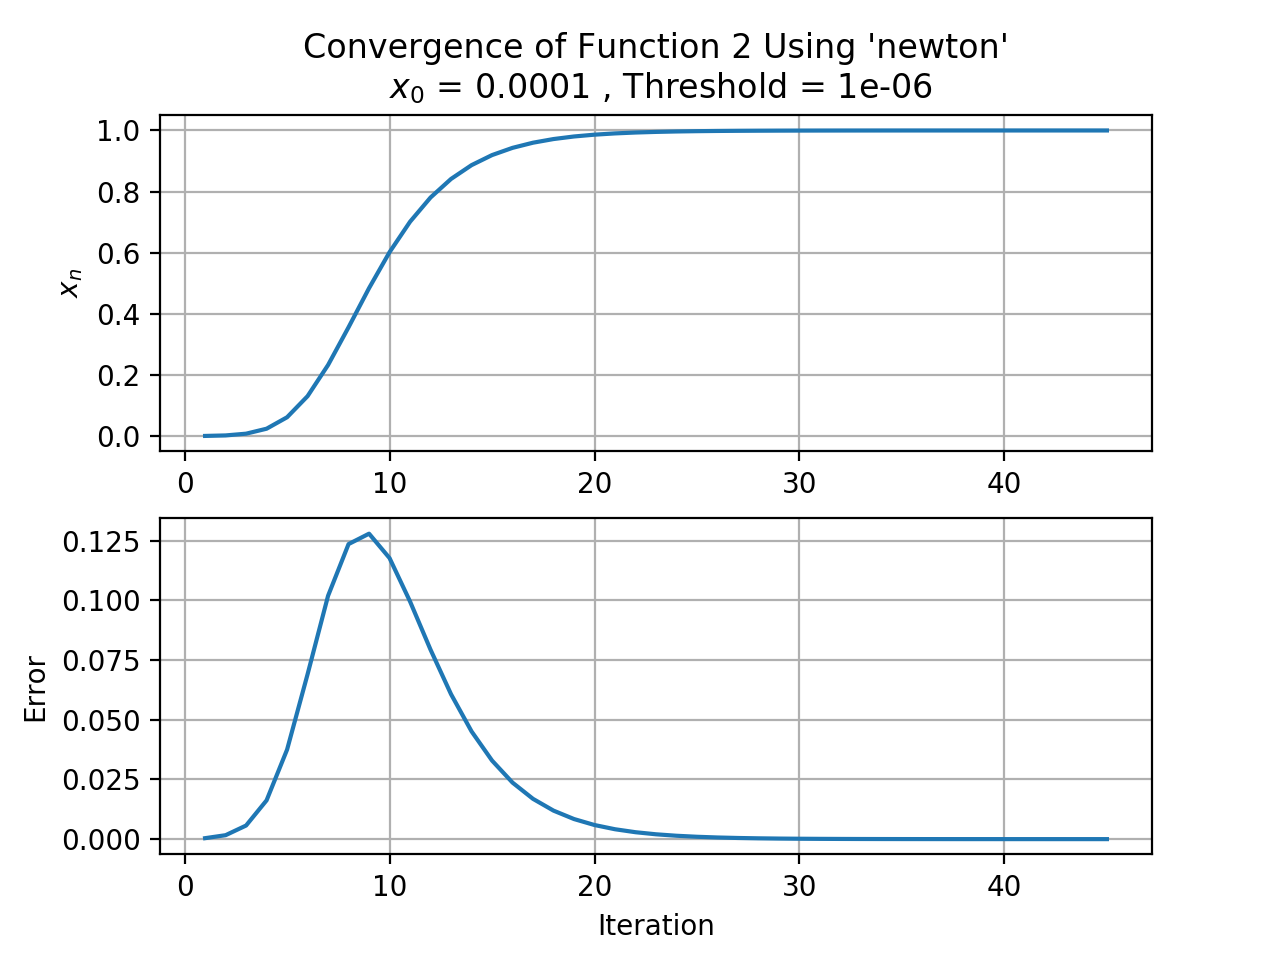
\includegraphics[width=1.0\textwidth]{./figures/initial_condition_2/result_2_1e-06.png}
		\label{fig:plot2dot3}
	\end{figure}
	
	\newpage
	For threshold  error 1.0e-8:
		\begin{figure}[h]
		\caption{The target function $f(x) = (x-1)\log_{10}(x)$.}
		\centering
		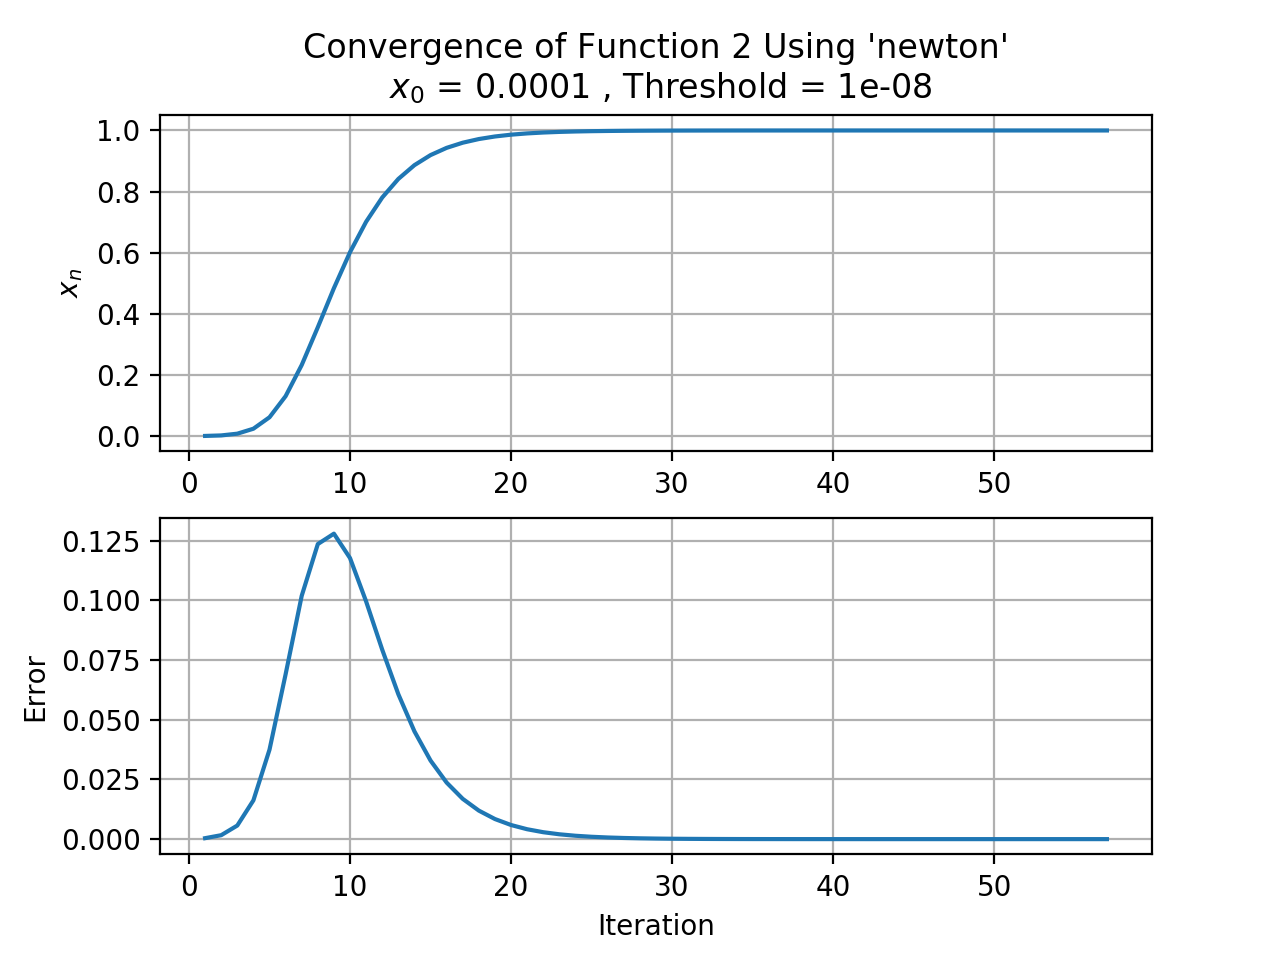
\includegraphics[width=1.0\textwidth]{./figures/initial_condition_2/result_2_1e-08.png}
		\label{fig:plot2dot3}
	\end{figure}







\end{document}